
% CF: you need to introduce this sectuon, what is profiling, why is it relevant to the project? what will this section be contributing?

% This study aim to speed up the computation implementation of a hippocampus model.
% The main problem with speeding up is knowing what to speed up.
% TODO define concept of a bottleneck
% explain Amdalh's law
% shows the effect speeding up some part on the whole system.
% Therefore, it is important to find the bottlenecks and speed them up one at a time.
% To enable this, Profilers are tools which do X Y and Z ...
% We need to choose a profiler.
% So we will review several options and select the one to use.

Our study is aiming to speed up the computational implementation of a hippocampus model.
But the main problem with speeding up software is knowing what should be targeted for speeding up.
The slower section of the code are known as bottlenecks, because they limit the number of operations that can be performed.
Amdahl's law describes the relationship between the parallelisable section and serial section of code.
\begin{equation}
    S_{latency}(s) = \frac{1}{(1-p)+\frac{p}{s}}
    \label{eqn:amdahl}
\end{equation}
The formalisation of Amdahl's law (as seen in \eqref{eqn:amdahl}), shows that the theoretical speed up is proportional to the amount of code that can be parallelised.
Therefore, it is important to find as many bottlenecks as possible, and speed them up one at a time.

To enable this, profilers are tools which monitor the process executing the program, and time individual calls to functions.
This is useful as it provides a numerical value to each function, including library calls, which can be used to identify the bottlenecks in the code.
In this section we compare different profilers, and select an profiler to use. 

\subsection{CPU profiling}
There are two modules for profiling in Python, \mono{Profile} and \mono{cProfile}.
The \mono{Profile} module is used for pure Python code, where as the \mono{cProfile} module is used for C-based Python code.
Both modules share the same interface and output format, thus the decision of using one over the other is dependent on speed.

As C is considered the most optimised language, moving a lot of our code into the C layer, which is done by the high level parallel libraries above, is important.
This makes the profiler of choice \mono{cProfile}, which can record and report functions that work in either the C layer or the Python layer.

The profiler provides six columns of information for the program, seen in \figureref{fig:pstats}.
These are:
\begin{itemize}
    \item Number of calls to the function (nCalls), which indicate the number of times a function is invoked,
    \item Total time spent in the function, excluding calls to other functions,
    \item Cumulative time spent in the function, including calls to other functions,
    \item Function name and location, which help identify where the profiled function in the code is.
    \item Two columns of the average time taken per call, for each of the types of timing.
\end{itemize}

% \picturesque{figures/lit_tools/profiling.png}{Sample output from the python profile module}{fig:pstats}

\begin{figure}[ht]
    \centering
    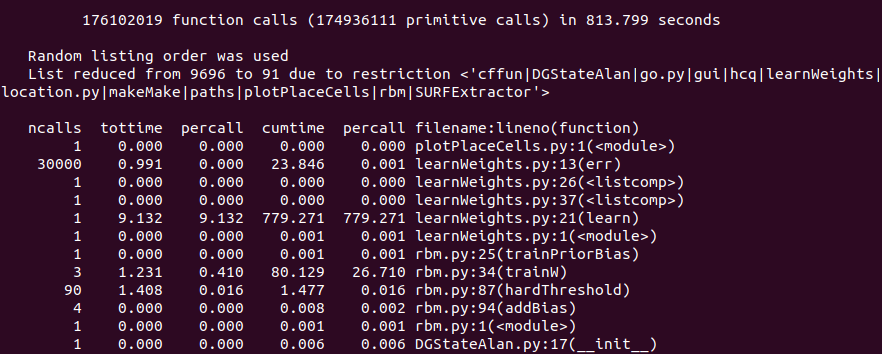
\includegraphics[width=0.8\textwidth]{figures/lit_tools/profiling.png}
    \caption{Sample output from the Python Profile module}
    \label{fig:pstats}
\end{figure}

At this level, we can disregard the cumulative time and average time columns as they do not definitively indicate slow areas of code.
This is because the slow parts of cumulative time can be attributed to a different function.
As for average times, by reducing the total time for the function to execute the average time will also fall.
The nCalls column is of less importance than the total time column as it does not actively contribute to identifying slow code, but can point to where our time should be focused in terms of optimisation.

As our goal is to reduce the global time for the system to learn, the total time column can be considered the most important measure of identifying optimisation possibilities.
This is because it ignores other factors and only reports the time taken, with respect to some overhead from the profiler tool.
By using the total time and nCalls metrics, it allows for more time to be spent on doing the refactoring and testing, as opposed to guessing where to optimise.




\subsubsection{Line Profiler}
Line profiler is a Python Library for profiling code on a line by line basis, instead of the entire software.
This allows for targeted profiling of the code.
The targeting of code profiling makes it useful for finding bottlenecks in identified functions.

% \wording

The Line profiler tool provides a percentage of the total time each line uses in the function.
This percentage is useful for identifying the bottlenecks, as a larger percentage indicates that more time is needed for a given line. 

An example of line by line profiling can be seen in \coderef{profiling:line_learn}.
Lines 10 through 14 only take a few microseconds, which has a negligible effect on the total percentage of time required.
However further down the function, lines 17-19, take approximately 18 seconds each, which is around 3.5\% of the total time, which points to optimising the \mono{trainW} function.
By optimising the \mono{trainW} function, we reduce the overall runtime of the \mono{learn} function, which aids our goal of optimising the learning process of the model.


The Line Profiler module is not part of the standard Python library.
It is only being maintained to current Python versions.
Thus it is not actively improved.
This may mean that it is not as accurate as the profiling modules.
Despite this, using it for identification purposes for large discrepancies in time for each line of the function.



\begin{minipage}{\linewidth}
\begin{lstlisting}[caption={Example output from the line profiler tool, showing part of the learn function of the model.}, label=profiling:line_learn]
Scale: 1e-6s
Total time: 529.294 s
File: /home/yakkus/github/jack-fork/hclearn/workspace/src/main/learnWeights.py
Function: learn at line 21

Line #      Hits         Time  Per Hit   % Time  Line Contents
==============================================================
    21                                           @profile
    22                                           def learn(path, dictSenses, dictGrids, N_mazeSize, ecs_gnd, dgs_gnd, ca3s_gnd, b_learnIdeal=True, b_learnTrained=False, b_learnDGWeights=True, learningRate=0.01):
    23         1          4.0      4.0      0.0      dghelper=None
    24  #Learn DG weights when you have visual input
    25         1          3.0      3.0      0.0      if b_learnDGWeights:
    26  #Extract data from dictionary of senses to train on 
    27         1         14.0     14.0      0.0          allSURFS = [ sense.surfs for sense in 
    ...
    59                                           
    60         1   19120224.0 19120224.0      3.6          WR = trainW(lag(hids,1), hids, WB, N_epochs=1, alpha=0.01)
    61         1   18793573.0 18793573.0      3.6          WS = trainW(senses,      hids, WB, N_epochs=1, alpha=0.01)
    62         1   17906180.0 17906180.0      3.4          WO = trainW(odom,        hids, WB, N_epochs=1, alpha=0.01)
\end{lstlisting}
\end{minipage}



\subsection{GPU profiling}

As with the low level parallelisation libraries, there is no set standard of profiling on a GPU, which is restricted by how it communicates with the CPU. 
This means that profilers for a given implementation, such as CUDA or OpenCL, only work for that implementation.
We look at the methods of profiling on different GPU architectures, as a reference for the benefits and drawbacks for each architecture for future work to consider.

\subsubsection{Profiling CUDA based software}
The CUDA parallel runtime uses two main software packages to handle parallel profiling: NSight Compute and NSight Systems.

NSight Compute profiles each CUDA kernel run, similar to the CPU profiling methods, which help identify which operations are the bottlenecks.
It also shows the dependencies of the kernels, such as a matrix multiplication kernel for input matrices of shape (m, k) and (k, n) using a vector multiplication kernel for each data point in the output matrix of shape (m, n).
It also shows how memory is used across the GPU, as it is faster to access local memory to a processing unit instead of global GPU memory. 
This is useful as CUDA kernels are C-based, meaning that it can help detect a memory leaks, however, in our case the CUDA kernels are managed via the Tensorflow library.
This particular feature is not useful to us at this time, however if further work is to directly use CUDA, then it would be necessary to ensure that the horizontal scaling of the model does not cause out of memory errors.

In contrast, NSight Systems looks at algorithm performance.
This can be considered the utilisation amount of the GPU and the amount of time waiting for threads to synchronise.
By understanding how the data is distributed across the GPU, it helps us understand whether a given function would benefit from being parallelised.
Parallel processing provides a better gain when there are as many compute units working on the same task as possible, as inactive or idle units do not aid the overall computation, which would increase the time taken.
By finding these inactive processing units, the algorithm can be optimised to reduce the amount of time a given processing unit has to wait for work to do.


{
% \textbf{\footnotesize{ROCm}}

% Tools: rocprof and roctracer

% basic about: https://github.com/ROCm-Developer-Tools/rocprofiler, https://rocmdocs.amd.com/en/latest/ROCm\_Tools/ROCm-Tools.html

% rocprof:
% \begin{itemize}
%     \item Spec: https://github.com/ROCm-Developer-Tools/rocprofiler/blob/amd-master/doc/rocprofiler\_spec.md
%     \item usage: https://github.com/ROCm-Developer-Tools/rocprofiler/blob/amd-master/doc/rocprof.md
%     \item per kernel output
%     \item has support for multiple gpus
%     \item mainly C++ only. Unlikely to have support for other languages
%     \item support for memory and thread management. useful for identifying which threads are under utilised, makes for more optimised code as fewer compute units are idle.
% \end{itemize}

% roctracer:
% \begin{itemize}
%     \item Spec: https://github.com/ROCm-Developer-Tools/roctracer/blob/amd-master/doc/roctracer\_spec.md
%     \item trace the call stack
%     \item mainly focuses on timing 
% \end{itemize}
}
\subsubsection{Profiling OpenCL based software}

Despite being an open standard, there is limited support for tools available to developers for profiling OpenCL software.
It is non-trivial to use NVidia's software for profiling OpenCL programs, as NSight Compute and NSight Systems are more suited to CUDA and Nvidia GPUs
AMD provides a software tool known as CodeXL, which is a part of the GPUOpen project \cite{gpuopen}.
This tool allows for the profiling and debugging of OpenCL kernels, which is useful as it helps to optimise the kernels used.
However it only works on AMD GPUs, where as our chosen framework, Tensorflow uses CUDA as its parallel backend.

OpenCL also has a built-in profiling tool which uses an event based system, however its functionality is limited.
This is because the events only register at significant points in an OpenCL kernel lifecycle.
Whilst it is useful for identifying a parallel function causing the bottleneck, it offers no further information on where a developer should begin looking to optimise.
This means that it is more suitable for this project to use NVidia software for profiling our parallel code due to its links to CUDA.



% As OpenCL is a standard as opposed to a proprietary runtime like CUDA, the information on profiling an OpenCL program is limited.
% This is due to profiling occurring within the OpenCL program instead of an external monitoring system.

% To profile in OpenCL, you need to enable event handling in the CL Command Queue.
% To profile a given kernel, we need to use the \mono{clGetEventProfilingInfo} Event on each OpenCL kernel we want to profile.
% This gives us a life cycle of the kernel, from before joining the execution queue to execution being completed.
% However it is only time based.
% Whilst this is the purpose of profiling, other platforms have extra features for helping to tune the kernel built into the tools.
% OpenCL does provide facilities for creating custom events, which can be used to profile individual threads or memory usage.
% The problem here is that developing and implementing these custom events reduces the overall time available for running experiments and working on optimising the original code.

